\documentclass{beamer}
\usetheme[bgphoto]{polimi}
\usepackage[utf8]{inputenc}
\usepackage{algorithm}
\usepackage{ifxetex}
\ifxetex
    \usepackage{fontspec}
    \setsansfont{Arial}[Scale=0.8]
\fi

\title{High Performance Scientific Computing for \\ Aerospace Project}
\subtitle{11th November 2025 update}
\date{November 11th, 2025}

\begin{document}
\begin{frame}
    \maketitle
\end{frame}


\begin{frame}{Slide 1}
    Content for slide 1 goes here.
\end{frame}

\begin{frame}{Input File}
\textbf{Structure of the input file:}
\begin{itemize}
    \item \textbf{Mesh points:} Number of points in X, Y, Z directions
    \begin{itemize}
        \item Example: \texttt{50 50 50} $\Rightarrow Nx=50, Ny=50, Nz=50$
    \end{itemize}
    
    \item \textbf{Time parameters:}
    \begin{itemize}
        \item \texttt{dt} - Time step size, e.g., \texttt{0.01}
        \item \texttt{T}  - Total simulation time, e.g., \texttt{10.0}
    \end{itemize}
    
    \item \textbf{Spatial step sizes:}
    \begin{itemize}
        \item \texttt{dx dy dz} - Grid spacing in X, Y, Z, e.g., \texttt{0.5 0.5 0.5}
    \end{itemize}
    
    \item \textbf{Initial conditions files:}
    \begin{itemize}
        \item \texttt{u0\_init\_file} - File with initial velocity values
        \item \texttt{p0\_init\_file} - File with initial pressure values
        \item \texttt{k\_file} - File with permeability values
    \end{itemize}
\end{itemize}
\end{frame}

\begin{frame}{Boundary conditions implementation}
    \begin{center}
        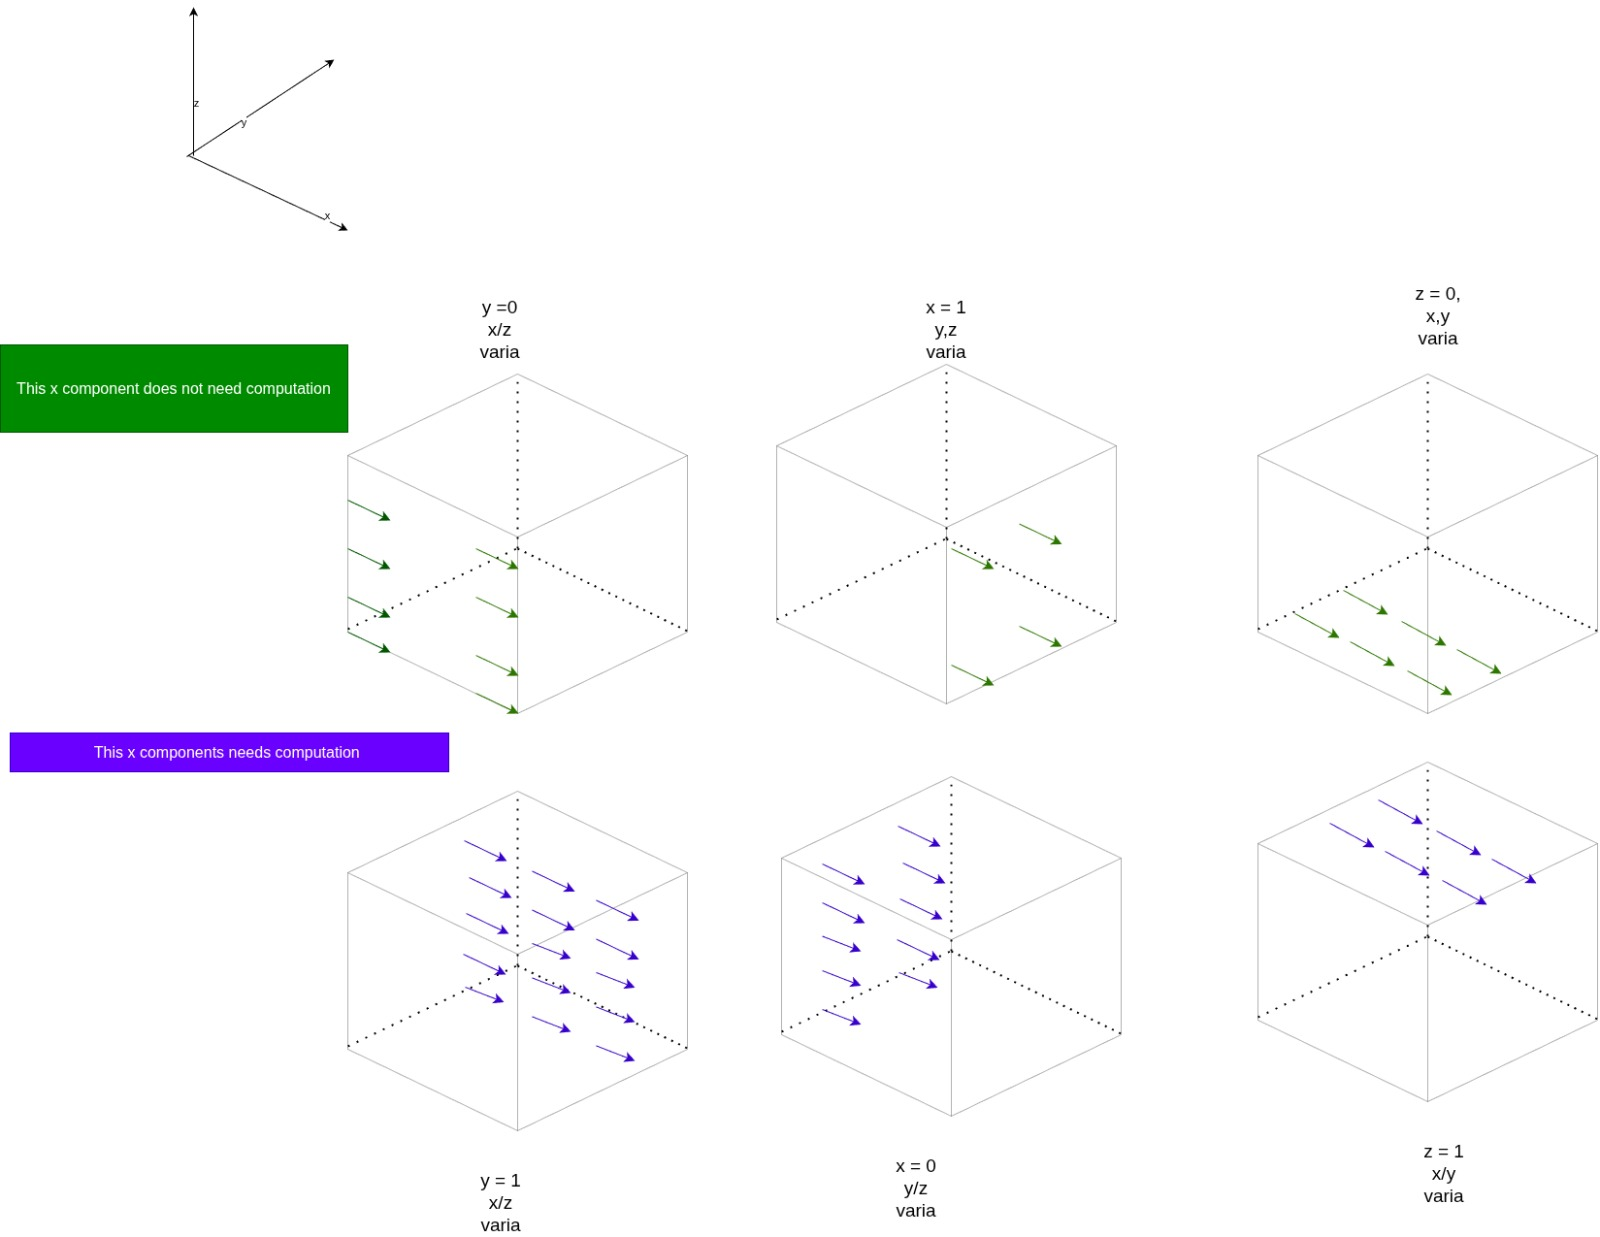
\includegraphics[width=0.9\textwidth,height=0.75\textheight,keepaspectratio]{img/boundary.jpeg}
    \end{center}
\end{frame}

\begin{frame}{Boundary conditions implementation pt.2}
    \begin{figure}
        \centering
        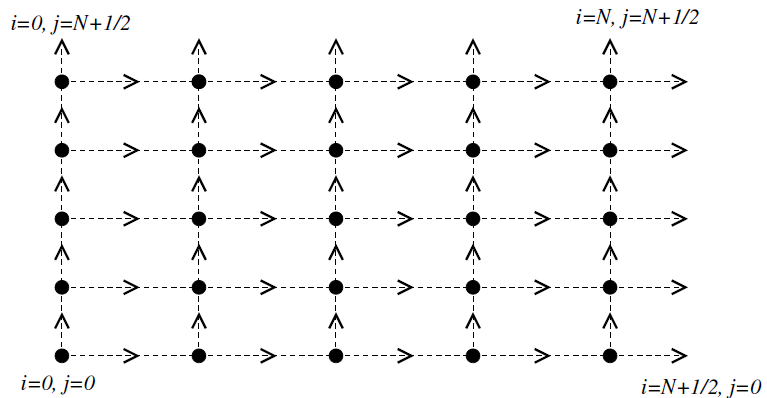
\includegraphics[width=\textwidth,height=0.5\textheight,keepaspectratio]{img/2DGrid.png}
    \end{figure}

\end{frame}

\begin{frame}{Future workflow}
    \begin{block}{Code Validation}
        \begin{itemize}
            \item Compute error
            \item Compute residual
            \item Convergence study
        \end{itemize}
    \end{block}
    
    \begin{block}{Parallelization Strategy}
        \begin{itemize}
            \item Vectorization of the sequential code
            \item Parallelization of the code
        \end{itemize}
    \end{block}
\end{frame}

\begin{frame}{Slide 5}
    Content for slide 5 goes here.
\end{frame}

\begin{frame}{Slide 6}
    Content for slide 6 goes here.
\end{frame}

\end{document}